\documentclass[a4paper,12pt]{article}

\usepackage[
    left=2cm,
    right=2cm,
    top=3cm,
    bottom=3cm
]{geometry}

\usepackage[utf8]{inputenc}
\usepackage[czech]{babel}
\usepackage[T1]{fontenc}
\usepackage{graphicx}
\usepackage{array}
\usepackage{booktabs}
\usepackage{tabularx}
\usepackage{makecell}
\usepackage{float}
\usepackage{newunicodechar}
\usepackage{url}
\usepackage{siunitx}
\usepackage{listings}
\usepackage{xcolor}
\usepackage{diagbox}
\usepackage{hyperref}
\usepackage{tikz}
\usepackage{pgfplots}
\pgfplotsset{compat=1.18}

\usepackage{fancyhdr}
\pagestyle{fancy}

\fancyhf{}
\fancyhead[L]{SME -- Lab 5: A/D převodníky}
\fancyhead[R]{Pavel Pernička}
\fancyfoot[C]{\thepage}

\fancypagestyle{firstpage}{
    \fancyhf{}
    \renewcommand{\headrulewidth}{0pt}
    \renewcommand{\footrulewidth}{0pt}
    \fancyfoot[C]{\thepage}
}

\definecolor{myblue}{RGB}{111,0,248}
\newcommand{\colorcircle}[1]{%
  \tikz[baseline=-0.6ex]\draw[fill=#1,draw=none] (0,0) circle (1.5ex);%
}
\newcommand{\unitC}{\,^\circ\mathrm{C}}
\newcommand{\unitV}{\,\mathrm{V}}
\newcommand{\unitA}{\,\mathrm{A}}
\newcommand{\units}{\,\mathrm{s}}
\newcommand{\unitmin}{\,\mathrm{min}}

\newcommand{\centered}[1]{\begin{tabular}{l} #1 \end{tabular}}

\addto\captionsczech{\renewcommand{\refname}{Seznam použité literatury}}
\addto\captionsczech{\renewcommand{\figurename}{\textbf{Obrázek}}}
\addto\captionsczech{\renewcommand{\tablename}{\textbf{Tabulka}}}
\renewcommand{\lstlistingname}{\textbf{Kód}}

\lstset{
    language=Python,
    basicstyle=\ttfamily\footnotesize,
    keywordstyle=\color{blue},
    commentstyle=\color{gray},
    stringstyle=\color{red},
    numbers=left,
    numberstyle=\tiny\color{gray},
    stepnumber=1,
    breaklines=true,
    frame=single
}

\begin{document}
\thispagestyle{firstpage}

\vspace*{\fill}
\begin{center}
\renewcommand{\arraystretch}{1.75}

\begin{tabularx}{\textwidth}{|X|X|X|}
    \hline
    \multicolumn{1}{|c|}{\rule{0pt}{2.25cm} 
\includegraphics[height=2cm]{img/ctu_logo.png}}
    & \multicolumn{2}{c|}{\makecell{\textbf{KATEDRA MĚŘENÍ}}} \\
    \hline
    \multicolumn{3}{|c|}{\Large \textbf{\centered{Senzory a měření}}} \\
    \hline
    \multicolumn{2}{|X}{\small{Jméno} \newline \textbf{Pavel Pernička}}
    & \multicolumn{1}{|X|}{\small{Datum měření} \newline \textbf{4.3.2026}} \\
    \hline
    {\small{Semestr} \newline \textbf{Letní 2026}}
    & {\small{Ročník} \newline \textbf{2.}}
    & {\small{Datum odevzdání} \newline \textbf{11.3.2026}} \\
    \hline
    \multicolumn{3}{|c|}{\rule{0pt}{1cm}} \\
    \hline
    \multicolumn{1}{|X|}{\small{Číslo úlohy \newline \textbf{5}}}
    & \multicolumn{2}{|p{9cm}|}{\small{Název úlohy \newline \textbf{A/D převodníky}}} \\
    \hline
\end{tabularx}

\end{center}
\vspace*{\fill}

\newpage
\pagestyle{fancy}
\section{Domácí příprava}
\begin{itemize}
  \item Seznamte s principem funkce integračního A/D převodníku, nakreslete základní blokové schéma. 
    \begin{itemize}
      \item Základní schéma je znázorněno na obrázku \ref{fig:integracni}.
      \item Do vstupu integrátoru po dobu $T_1$ necháme připojené měřené napětí.
      \item Po uplynutí doby $T_1$ přepneme vstup na referenční napětí s opačnou polaritou oproti měřenému, deintegrujeme a začínáme počítat čas $T_2$.
      \item Jakmile pomocí komparátoru zaznamenáme průchod nulou, změříme čas $T_2$.
      \item Ze znalosti $T_1$, $T_2$ a $U_{\mathrm{ref}}$ vypočítáme měřené napětí.
    \end{itemize}
  \item Odvoďte rovnici pro výpočet měřeného napětí z doby deintegrace (při znalosti referenčního napětí a doby integrace měřeného napětí). Záleží výpočet na časové konstantě integrátoru? Případně jak?
    \begin{itemize}
      \item $U_{\mathrm{measured}} = U_{\mathrm{ref}} \cdot \frac{T_2}{T_1}$.
      \item Výpočet na časové konstantě $\tau$ integrátoru nezáleží, protože se při deintegraci vyruší. Roli by hrála jedině tehdy, pokud by se mezi integrací a deintegrací změnila.
    \end{itemize}
  \item Z jakých obvodů se v principu skládá převodník s postupnou aproximací?
    \begin{itemize}
      \item Z registru, D/A převodníku, který převádí bity v registru na napětí, a komparátoru.
    \end{itemize}
  \item Který bit je při sériové komunikaci aproximačních A/D převodníků (např. ADS8512) posílán jako první (MSB, nebo LSB) a proč?
    \begin{itemize}
      \item Protože MSB odpovídá polovině rozsahu A/D převodníku. SAR v principu dělá binární vyhledávání, jehož prvním krokem je rozpůlit interval.
    \end{itemize}
  \item Na jakou hranu hodin je platná hodnota výstupního bitu sériového výstupu převodníku ADS8512?
    \begin{itemize}
      \item Na \textit{rising edge} (dle datasheetu).
    \end{itemize}
\end{itemize}

\begin{figure}[H]
\centering
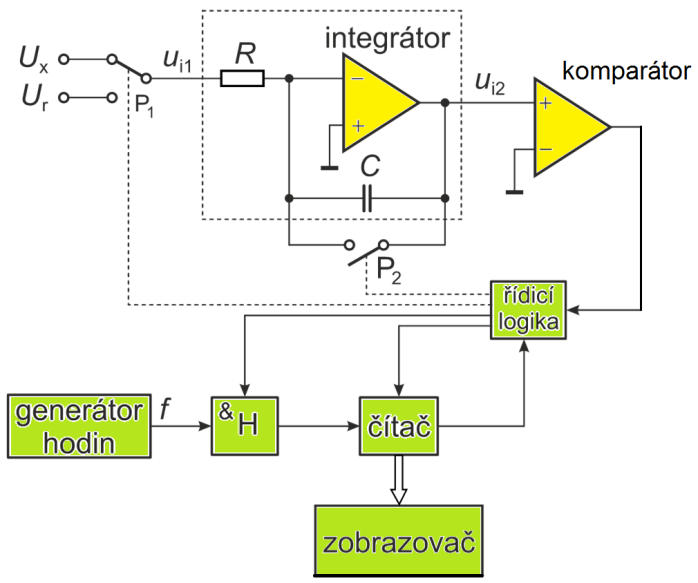
\includegraphics[width=0.75\textwidth]{img/integracni.png}
\caption{Schéma zapojení integračního A/D převodníku}
\label{fig:integracni}
\end{figure}

\section{Měření}
\subsection{Signál z integračního převodníku}
Popište průběhy zobrazené na osciloskopu pro integrační převodník --- kdy dochází k integraci vstupního napětí, kdy referenčního a co je měronosnou veličinou. Nastavte na vstup převodníku např. napětí $4\,\mathrm{V}$, bez připojeného rušení a s dobou integrace $20\,\mathrm{ms}$; pro přípravu se podívejte na obr.~2 z návodu.

Průběh je znázorněn na obrázku \ref{fig:integracni_1}. Jednotlivé části jsou:
\begin{enumerate}
  \item nulování,
  \item integrace,
  \item deintegrace,
  \item integrace šumu, když zrovna neprobíhá měření.
\end{enumerate}

\begin{figure}[H]
\centering
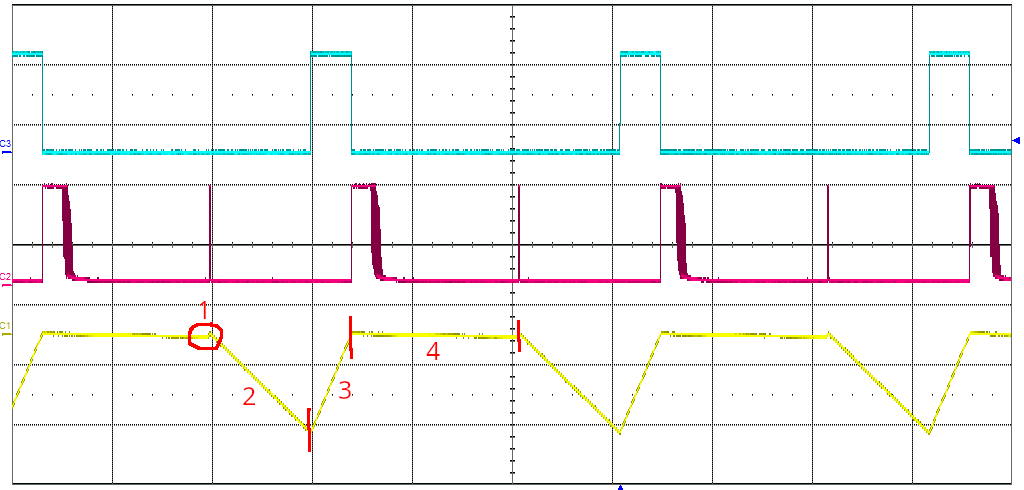
\includegraphics[width=0.95\textwidth]{img/integracni_1.png}
\caption{Naměřený průběh napětí integrátoru}
\label{fig:integracni_1}
\end{figure}

\subsection{Časová konstanta integrátoru}
Vhodným měřením určete časovou konstantu integrátoru. Při znalosti odporu v integrátoru ($1\,\mathrm{M\Omega}$) určete kapacitu integračního kondenzátoru.

Pro výpočet časové konstanty $\tau$ využijeme následující vztah:
$$
\frac{dV_{\mathrm{out}}}{dt} = -\frac{V_{\mathrm{in}}}{RC}
$$

$$
\tau = RC = \frac{V_{\mathrm{in}}}{\left|\frac{dV_{\mathrm{out}}}{dt}\right|}
$$

Naměřili jsme $V_{\mathrm{in}} = 3{,}94\,\mathrm{V}$ a časová derivace $V_{\mathrm{out}}$ je zkrátka sklon integrační přímky. Změnu napětí a času jsme určili pomocí kurzorů:
$$
\frac{dV_{\mathrm{out}}}{dt} = \frac{-0{,}817}{0{,}0202} = -40{,}4
$$

A tedy:
$$
\tau = \frac{3{,}94}{40{,}4} = 98\,\mathrm{ms}
$$

Kapacitu určíme díky znalosti odporu v integrátoru $R = 1\,\mathrm{M\Omega}$ a nyní i časové konstanty jako:
$$
C = \frac{\tau}{R} = \frac{0{,}098}{1 \cdot 10^{6}} = 97{,}5\,\mathrm{nF}
$$

\subsection{Periodický rušivý signál}
Ověřte vliv (nebo naopak potlačení) střídavého rušení na měření stejnosměrného napětí. Na vstup přiveďte $4\,\mathrm{VDC}$ a na vstup \uv{noise} přiveďte $4\,\mathrm{V_{P-P}}$, $50\,\mathrm{Hz}$ sinusový signál z generátoru. Jaké frekvence rušivého signálu budou potlačeny při nastavené době integrace $100\,\mathrm{ms}$? Proč je rozumná doba integrace v násobcích $20\,\mathrm{ms}$ (v Evropě)?

Pokud má rušení frekvenci $50\,\mathrm{Hz}$, tak při nastavené době integrace v násobcích $20\,\mathrm{ms}$ jej nepozorujeme, jelikož $20\,\mathrm{ms}$ je perioda tohoto signálu, tedy průměrná hodnota je nulová. Naměřený signál vypadá obdobně jako na obrázku \ref{fig:integracni_1}. Pokud dobu integrace pomocí přepínačů nastavíme mimo násobek periody, pozorujeme zvlnění signálu, jako je tomu na obrázku \ref{fig:integracni_2}.

\begin{figure}[H]
\centering
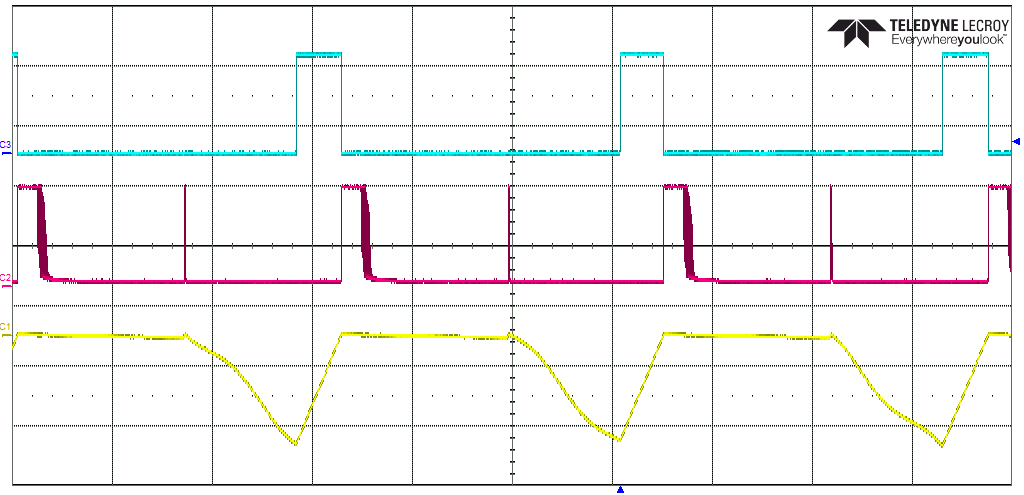
\includegraphics[width=0.95\textwidth]{img/integracni_2.png}
\caption{Naměřený průběh napětí integrátoru se zapnutým rušením a $T_1$ mimo násobek periody}
\label{fig:integracni_2}
\end{figure}

\subsection{Seznámení s osciloskopem}
Seznamte se s obsluhou digitálního osciloskopu MSO4000 s integrovaným logickým analyzátorem, tj. jak se nastavuje mód jednoho odběru (\textit{single}) a opakované měření, jak se mění nastavení časové základny a zesílení analogového kanálu, jak lze zapnout a vypnout jeden z digitálních kanálů logického analyzátoru a jak lze uložit aktuální obraz na obrazovce do souboru na USB flash disku.

Ovládání je poměrně krkolomně vymyšlené.

\subsection{Aproximační A/D převodník v polovině rozsahu}
Zobrazte na obrazovce osciloskopu časové průběhy na výstupech a řídicích vstupech diskrétního aproximačního A/D převodníku pro dvě napětí v okolí hodnoty $5\,\mathrm{V}$ (např. $4{,}97\,\mathrm{V}$ a $5{,}03\,\mathrm{V}$, tedy hodnoty okolo poloviny rozsahu). Sledujte paralelní výstup $D_0$ až $D_7$, sériový výstup $S_{\mathrm{BUSY}}$, $S_{\mathrm{CLK}}$ a $S_{\mathrm{DAT}}$. Pomocí analogových kanálů osciloskopu zobrazte vstupní napětí $V_{\mathrm{in}}$, výstup interního D/A převodníku $V_{\mathrm{DAC}}$ a výstup interního komparátoru $V_{\mathrm{COMP}}$. Zobrazení uložte s pomocí funkce \texttt{PRINT} na osciloskopu na USB flash disk a po případné úpravě jej vložte do protokolu o měření.

Můžeme pozorovat přechod MSB na logickou $1$ při přesažení poloviny rozsahu. Napětí $4{,}98\,\mathrm{V}$ je reprezentováno jako $01111111$ a $5{,}01\,\mathrm{V}$ jako $10000000$.
 
\begin{figure}[H]
\centering
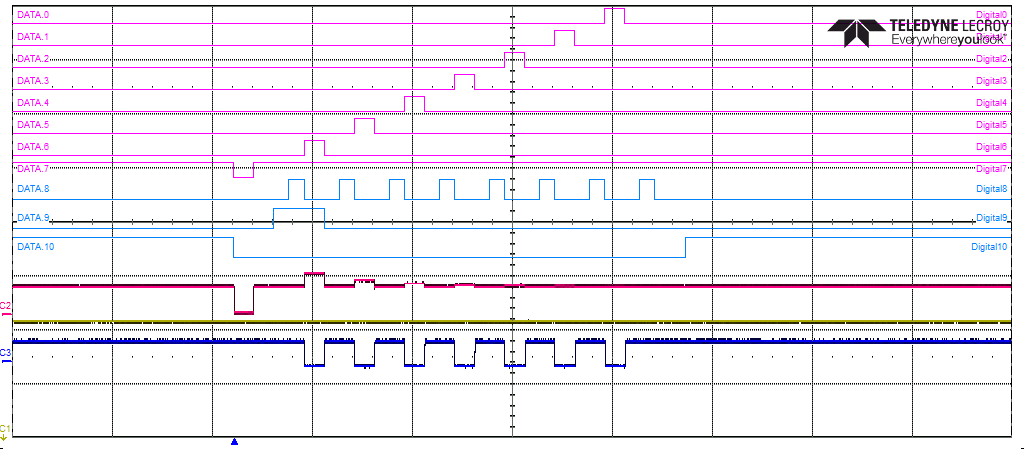
\includegraphics[width=0.95\textwidth]{img/above_5.png}
\caption{Signály aproximačního převodníku při $U_x = 5{,}01\,\mathrm{V}$ (binárně $128$)}
\label{fig:above5}
\end{figure}

\begin{figure}[H]
\centering
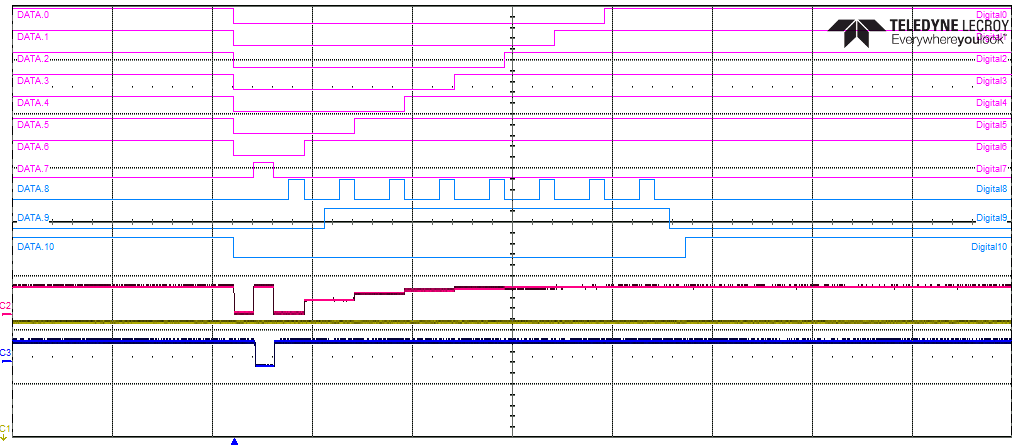
\includegraphics[width=0.95\textwidth]{img/bellow_5.png}
\caption{Signály aproximačního převodníku při $U_x = 4{,}98\,\mathrm{V}$ (binárně $127$)}
\label{fig:bellow5}
\end{figure}

\subsection{Převodní charakteristika}
Změřte převodní charakteristiku převodníku pro $8$ a více hodnot z celého rozsahu A/D převodníku ($0$ až $10\,\mathrm{V}$), např. pro $0{,}000\,\mathrm{V}$, $0{,}060\,\mathrm{V}$, $1{,}000\,\mathrm{V}$, $2{,}500\,\mathrm{V}$, $5{,}000\,\mathrm{V}$, $7{,}500\,\mathrm{V}$, $9{,}000\,\mathrm{V}$ a $9{,}9\,\mathrm{V}$. Naměřené charakteristiky A/Č převodníků porovnejte s ideální charakteristikou a vyneste do grafu odchylky.

Naměřené hodnoty jsou pro jednotlivá napětí uvedeny v tabulce \ref{fig:table}. V grafu \ref{fig:char} je srovnání naměřené charakteristiky a ideálního, dokonale lineárního stavu. V grafu \ref{fig:odchylka} jsou odchylky mezi naměřenými a ideálními hodnotami.

\begin{table}[H]
\centering
\begin{tabular}{|c|c|c|c|c|c|c|c|c|}
\hline
$V_{\mathrm{in}}$ [V] & 0 & 0.060 & 1.0 & 2.5 & 5.0 & 7.5 & 9.0 & 9.9 \\
\hline
Digitální hodnota & 0 & 1 & 25 & 64 & 128 & 192 & 231 & 254 \\
\hline
\end{tabular}
\caption{Naměřená převodní charakteristika aproximačního převodníku}
\label{fig:table}
\end{table}

\begin{figure}[H]
\centering
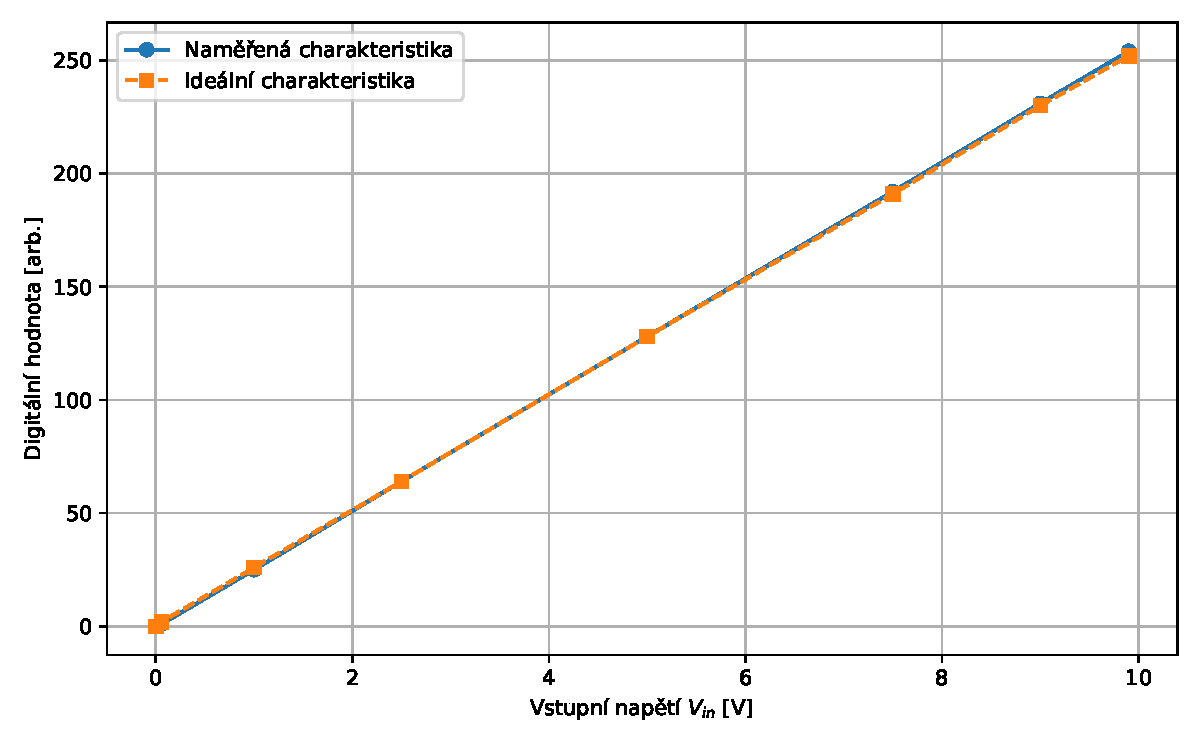
\includegraphics[width=0.95\textwidth]{img/char.pdf}
\caption{Srovnání naměřených a ideálních hodnot z aproximačního A/D převodníku}
\label{fig:char}
\end{figure}

\begin{figure}[H]
\centering
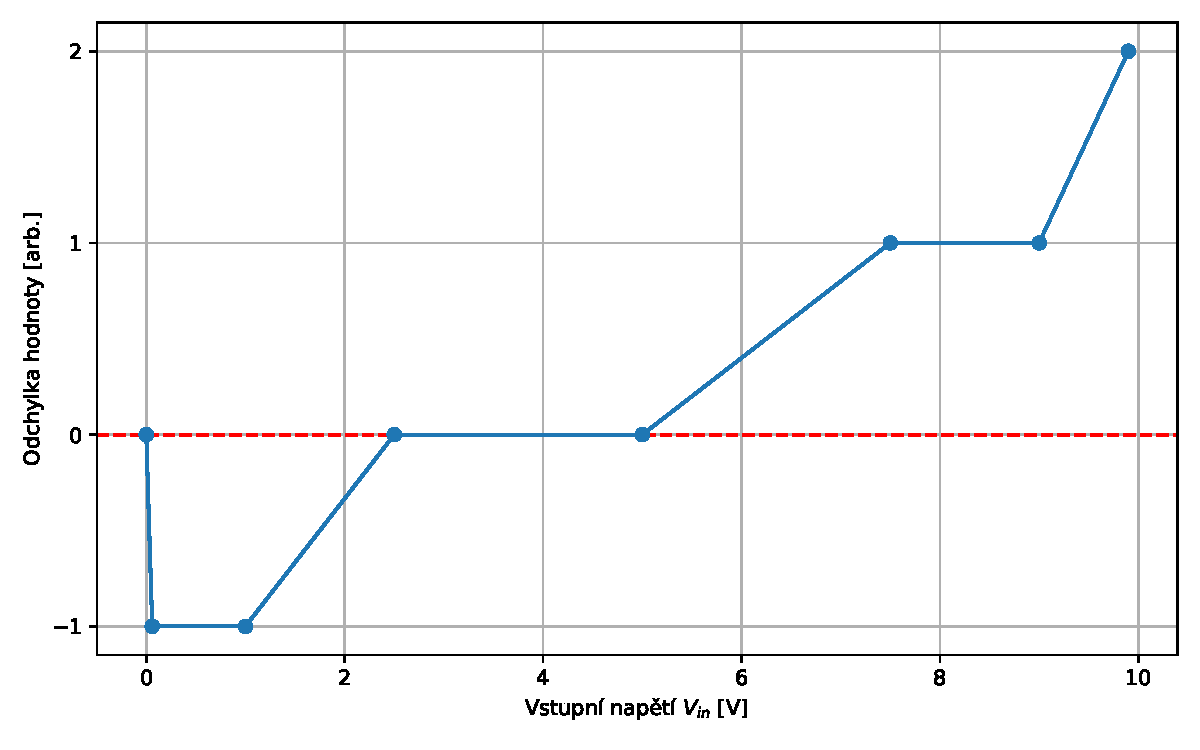
\includegraphics[width=0.95\textwidth]{img/odchylka.pdf}
\caption{Odchylky mezi naměřenými a ideálními hodnotami z aproximačního A/D převodníku}
\label{fig:odchylka}
\end{figure}

\end{document}
